109. $y=\cfrac{x^2-10x+24}{|x-7|+|x-3|-2}=\begin{cases}
\cfrac{(x-6)(x-4)}{7-x+3-x-2}=\cfrac{6-x}{2},\ x<3,\\
\cfrac{(x-6)(x-4)}{7-x+x-3-2}=\cfrac{x^2-10x+24}{2},\ 3\leqslant x \leqslant 7,\\
\cfrac{(x-6)(x-4)}{x-7+x-3-2}=\cfrac{x-4}{2},\ 7<x.\end{cases}$
$$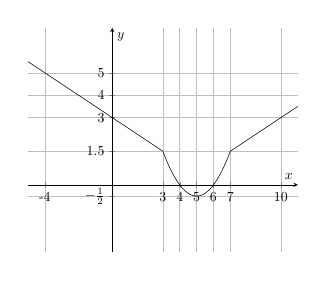
\begin{tikzpicture}[scale=0.5]
\begin{axis}[
    axis lines = middle,
    grid=major,
    legend pos={south west},
    xlabel = {$x$},
    ylabel = {$y$},
    ymin=-3,
    ymax=7,
    xtick={-4, 3 , 5, 7, 10, 4, 6},
    xticklabels={-4, 3 , 5, 7, 10, 4, 6},
    ytick={ 5, 4,  -0.5, 1.5,3},
    yticklabels={  5, 4,  $-\frac{1}{2}$, 1.5,3}           ]
\addplot[domain=-5:3, samples=100, color=black] {(6-x)/2};
\addplot[domain=3:7, samples=100, color=black] {(x*x-10*x+24)/2};
\addplot[domain=7:11, samples=100, color=black] {(x-4)/2};
%\addplot[domain=-3.1:2.5, samples=100, color=red] {70*abs(1-2*abs(abs(x)-2))-10*x^2+10*x-70};
	%\addlegendentry{$\text{Рис. 1}$};
\end{axis}
\end{tikzpicture}$$
